% Spectrum and frame -- working notes, Part I. Build instructions: README.md in this folder.
% Numbers from synthetic computations come from generated/numbers.tex (written by make_figures.py).
\documentclass[11pt,a4paper]{article}

\usepackage[T1]{fontenc}
\usepackage{lmodern}
\usepackage[a4paper,margin=2.6cm]{geometry}
\usepackage{amsmath,amssymb,amsthm,mathtools}
\usepackage{graphicx}
\usepackage{booktabs}
\usepackage[shortlabels]{enumitem}
\usepackage{xcolor}
\usepackage{microtype}
\usepackage[colorlinks=true,linkcolor=blue!50!black,urlcolor=blue!50!black,citecolor=blue!50!black]{hyperref}

% Generated by make_figures.py; do not edit by hand.
\newcommand{\NumSimDim}{2{,}000}
\newcommand{\NumSimEtaScaled}{8.9}
\newcommand{\NumSimFrob}{0.020}
\newcommand{\NumKvecSim}{169}
\newcommand{\NumKvecPred}{166}
\newcommand{\NumKvalSim}{1{,}801}
\newcommand{\NumKvalWeyl}{560}
\newcommand{\NumKvecWorst}{8.4}
\newcommand{\NumNeighbourRank}{25}
\newcommand{\NumRelValTopScaled}{3.4}
\newcommand{\NumHardSixteen}{0.007}
\newcommand{\NumHardTwoHundred}{0.12}
\newcommand{\NumHardThousand}{0.54}
\newcommand{\NumSoftSixteen}{0.0739}
\newcommand{\NumSoftTwoHundred}{0.183}
\newcommand{\NumSoftThousand}{0.214}
\newcommand{\NumSoftCuts}{15{,} 193 and 917}
\newcommand{\NumCrossCut}{346}
\newcommand{\NumShareSixForty}{0.480}
\newcommand{\NumShareFourK}{0.380}
\newcommand{\NumShareSixteenK}{0.329}
\newcommand{\NumShareThreeK}{0.393}
\newcommand{\NumKantFourK}{4.45}
\newcommand{\NumFrameParamsFourK}{8{,}386{,}560}
\newcommand{\NumKantSixteenK}{5.14}
\newcommand{\NumFrameParamsSixteenK}{134{,}209{,}536}
\newcommand{\NumHaarRelSd}{0.203}
\newcommand{\NumHaarMCDraws}{200{,}000}
\newcommand{\NumHaarMCVarRatio}{1.0016}
\newcommand{\NumHaarMCMeanRatio}{0.9995}
\newcommand{\NumDdeltaExact}{1570.2}
\newcommand{\NumDdeltaAsym}{1570.8}
\newcommand{\NumDdeltaLogExact}{1628.1}
\newcommand{\NumDdeltaLogAsym}{1628.5}
\newcommand{\NumKronSlope}{0.77}
\newcommand{\NumKronPred}{0.75}
\newcommand{\NumDirWithinTen}{0.24}
\newcommand{\NumTraceWithinTen}{0.329}
\newcommand{\NumDirWithinThousand}{24}
\newcommand{\NumTraceWithinThousand}{0.842}
\newcommand{\NumTailBoundTwo}{0.038}
\newcommand{\NumTailTrueTwo}{0.037}
\newcommand{\NumTwoShift}{0.0062}
\newcommand{\NumTwoAngle}{31.7}
\newcommand{\NumKantWorstFourK}{1{,}025}


\newcommand{\R}{\mathbb{R}}
\newcommand{\E}{\mathbb{E}}
\newcommand{\Orth}{\mathrm{O}}
\newcommand{\Sym}{\mathbb{S}}
\DeclareMathOperator{\tr}{tr}
\DeclareMathOperator{\diag}{diag}
\DeclareMathOperator{\Var}{Var}
\DeclareMathOperator{\Cov}{Cov}
\DeclareMathOperator{\Dir}{Dirichlet}
\DeclarePairedDelimiter{\norm}{\lVert}{\rVert}
\DeclarePairedDelimiter{\abs}{\lvert}{\rvert}
\DeclarePairedDelimiter{\floor}{\lfloor}{\rfloor}
\newcommand{\op}{\mathrm{op}}
\newcommand{\F}{\mathrm{F}}
\newcommand{\study}[1]{\path{#1}}
\newcommand{\evL}{\textsc{[l]}}

\theoremstyle{plain}
\newtheorem{proposition}{Proposition}[section]
\newtheorem{lemma}[proposition]{Lemma}
\newtheorem{corollary}[proposition]{Corollary}
\theoremstyle{definition}
\newtheorem{definition}[proposition]{Definition}
\newtheorem{approximation}[proposition]{Approximation}
\newtheorem{example}[proposition]{Example}
\theoremstyle{remark}
\newtheorem{remark}[proposition]{Remark}
\newtheorem{observation}[proposition]{Observation}
\newtheorem{question}{Question}

\title{Spectrum and frame\\[0.3em]
\large A probabilistic view of the curvature that preconditioned optimizers estimate\\[0.2em]
Part I: What a power-law spectrum of a PSD matrix means}
\author{Working notes --- G.~Tirpitz and Claude (Opus 5.5)}
\date{Started 23 October 2026 \quad (version 0.1)}

\begin{document}
\maketitle

\begin{abstract}
These notes build, from first principles and in stages, a probabilistic model of the curvature matrices that
preconditioned optimizers such as SOAP estimate. The organising idea is to split a positive semi-definite matrix
into its \emph{spectrum}, a distribution of eigenvalues, and its \emph{frame}, its eigenvectors. The lab's
measurements show the first nearly stationary and the second rotating late in training. Part~I treats one fixed
matrix. It makes precise what a power-law spectrum is (four equivalent forms), what the exponent decides (which
functionals are set by the top of the spectrum and which by the tail), how the spectrum becomes a probability
distribution once the frame is unknown, and what a power law implies about the frame: eigenvalues are resolved far
deeper than eigenvectors. It closes with what the literature already contains and with the questions that open
Part~II.
\end{abstract}

\tableofcontents

%======================================================================
\section{Why these notes}
%======================================================================

Three results from the lab's CIFAR-10 studies (a depth-6 ViT; per-tensor generalized Gauss--Newton (GGN) blocks)
motivate them.
\begin{enumerate}[(1)]
\item Late in training the per-tensor GGN spectrum is a nearly fixed power law with exponent $\alpha\approx 1$, while
  its eigenvectors rotate. A top-16 subspace cached 10 steps earlier keeps only 0.84--0.88 of the current top-16
  curvature (\study{spectral_rotation_20261020}, \evL).
\item A spectrum alone cannot precondition the bulk of the spectrum: a power-law diagonal reaches only the level of
  the exact diagonal. A few curvature products can (\study{bulk_krylov_20261014}, \evL).
\item The best power of the curvature falls from about $3/4$ early in training to $1/2$ late, as the noise scales of
  strongly preconditioned steps grow (\study{noise_scale_20261021}, \evL).
\end{enumerate}
SOAP already has the structure the first result suggests: an eigenbasis refreshed rarely (every 10 steps in our
runs) and a diagonal second-moment estimate refreshed every step. The question behind these notes is whether SOAP
was built from a model of how spectrum and frame evolve. If not, can such a model explain SOAP and improve it, for
example by forecasting when to refresh the frame, how long to average, and how to treat momentum? Section~\ref{sec:known}
summarises what we found. SOAP's design is motivated by computational cost and by experiments, and we found no
dynamical model of spectrum and frame behind it or elsewhere.

\paragraph{Programme.}
\begin{description}[leftmargin=1.2em]
\item[Part I] (this note): one PSD matrix. Spectrum and frame, power laws, the spectrum as a probability
  distribution, and what a power law implies about the frame.
\item[Part II]: dynamics. Matrices that move on or near the set of matrices with a fixed spectrum; drift and
  diffusion of the frame; models and their fingerprints in the lab's data.
\item[Part III]: inference. Priors with a known spectrum and an unknown frame; Krylov methods as inference on
  spectral measures; a stale frame with a fresh diagonal (EKFAC, SOAP) as an estimator.
\item[Part IV]: control. Forecasting refresh times, averaging windows and the treatment of momentum.
\end{description}

\paragraph{Conventions.}
Labels follow the lab's writing rules. \emph{Propositions}, \emph{lemmas} and \emph{corollaries} are exact
statements with proofs. \emph{Approximations} are asymptotic or first-order statements with their conditions.
\emph{Observations} are measurements; they name the study and carry the evidence level \evL{} (local, at fixed
states) or \textsc{[t]} (training). Numbers from synthetic computations are produced by \texttt{make\_figures.py} in
this folder; numbers from the lab's studies are taken from the studies' \texttt{RESULTS.md} files.

\paragraph{Notation.}
$\Sym^D$ is the set of real symmetric $D\times D$ matrices and $\Sym^D_+$ its positive semi-definite (PSD) subset;
$\Orth(D)$ is the orthogonal group. Eigenvalues are sorted, $\lambda_1\ge\dots\ge\lambda_D$. $\norm{\cdot}_\op$ is
the operator norm and $\norm{\cdot}_\F$ the Frobenius norm. $\delta_x$ is the point mass at $x$, $H_n=\sum_{k\le
n}1/k$ the harmonic number, $\zeta$ the Riemann zeta function and $\gamma\approx0.5772$ Euler's constant.

%======================================================================
\section{A PSD matrix is a spectrum and a frame}\label{sec:frame}
%======================================================================

\begin{definition}[Spectrum and frame]
Every $A\in\Sym^D_+$ can be written $A=U\Lambda U^\top$ with $U\in\Orth(D)$ and
$\Lambda=\diag(\lambda_1,\dots,\lambda_D)$, $\lambda_1\ge\dots\ge\lambda_D\ge0$. The vector
$\sigma(A)=(\lambda_1,\dots,\lambda_D)$ is the \emph{spectrum} of $A$. Any such $U$ is a \emph{frame} of $A$; its
columns $u_k$ are eigenvectors.
\end{definition}

\begin{proposition}[The orbit of a spectrum]\label{prop:orbit}
Fix $\Lambda$.
\begin{enumerate}[(a)]
\item The set $\mathcal{O}_\Lambda=\{Q\Lambda Q^\top: Q\in\Orth(D)\}$ is the set of PSD matrices with spectrum
  $\sigma=(\lambda_1,\dots,\lambda_D)$.
\item If the $\lambda_k$ are distinct, the frame of $A\in\mathcal{O}_\Lambda$ is unique up to the signs of its columns,
  and $\mathcal{O}_\Lambda$ is a manifold of dimension $D(D-1)/2$.
\item If the distinct values have multiplicities $m_1,\dots,m_r$, the frame is unique up to
  $\Orth(m_1)\times\dots\times\Orth(m_r)$ acting within the eigenspaces, and
  $\dim\mathcal{O}_\Lambda=D(D-1)/2-\sum_j m_j(m_j-1)/2$.
\end{enumerate}
\end{proposition}
\begin{proof}
(a) is the spectral theorem. The stabiliser $\{Q: Q\Lambda Q^\top=\Lambda\}$ consists of the $Q$ that commute with
$\Lambda$, that is, that map every eigenspace to itself. These form $\Orth(m_1)\times\dots\times\Orth(m_r)$, which is
the finite group of diagonal sign matrices when all $m_j=1$. The orbit is the homogeneous space $\Orth(D)$ modulo
the stabiliser, of dimension $\dim\Orth(D)-\sum_j\dim\Orth(m_j)=D(D-1)/2-\sum_j m_j(m_j-1)/2$.
\end{proof}

\begin{example}[Counting]\label{ex:count}
For the $64\times64$ weight blocks of the lab's ViT ($D=4{,}096$) the spectrum is $4{,}096$ numbers and the frame
\NumFrameParamsFourK. For the $64\times256$ blocks ($D=16{,}384$) they are $16{,}384$ and \NumFrameParamsSixteenK. A
power-law fit compresses the spectrum to two or three numbers. ``The spectrum is stable'' therefore constrains a
vanishing part of the matrix; almost all of its information is in the frame.
\end{example}

\begin{definition}[Invariant and equivariant maps]
A function $F:\Sym^D\to\R$ is \emph{invariant} if $F(QAQ^\top)=F(A)$ for all $Q\in\Orth(D)$. A map
$G:\Sym^D\to\Sym^D$ is \emph{equivariant} if $G(QAQ^\top)=Q\,G(A)\,Q^\top$ for all $Q\in\Orth(D)$.
\end{definition}

\begin{proposition}\label{prop:equivariant}
\begin{enumerate}[(a)]
\item $F$ is invariant if and only if $F(A)$ depends on $A$ only through $\sigma(A)$.
\item If $G$ is equivariant and $A$ has distinct eigenvalues, then $G(A)=\sum_k\varphi_k u_ku_k^\top$ for some
  numbers $\varphi_k$. In particular $G(A)$ commutes with $A$, and $G(A)=p(A)$ for a polynomial $p$ of degree less
  than $D$ (which may depend on $A$).
\end{enumerate}
\end{proposition}
\begin{proof}
(a) $A=U\diag(\sigma(A))U^\top$, so invariance gives $F(A)=F(\diag\sigma(A))$; the converse is immediate.
(b) The reflection $R_k=I-2u_ku_k^\top$ satisfies $R_kAR_k^\top=A$, so equivariance gives $G(A)=R_kG(A)R_k$ and
hence $R_k\bigl(G(A)u_k\bigr)=G(A)R_ku_k=-G(A)u_k$. The $-1$ eigenspace of $R_k$ is $\mathrm{span}(u_k)$, so
$G(A)u_k=\varphi_ku_k$. Since the $\lambda_k$ are distinct, Lagrange interpolation gives $p$ with
$p(\lambda_k)=\varphi_k$.
\end{proof}

\begin{remark}[What this means for us]\label{rem:invariance}
Every statement about ``the spectrum'' (a power law, a trace, a condition number) is an invariant function. It
takes the same value on the whole orbit and carries no information about the frame. Conversely, a preconditioner
that must not depend on an unknown frame has to be equivariant, hence a function of the current matrix. Such a map is
applied with matrix--vector products and never needs eigenvectors. Krylov methods (CG, Lanczos) are of this kind,
equivariant jointly in the matrix and the start vector; a stored eigenbasis (SOAP, PARSEC-L) is not.
\end{remark}

%======================================================================
\section{The spectral distribution, and four faces of a power law}\label{sec:faces}
%======================================================================

\begin{definition}[Spectral distribution, counting function, rank function]
The \emph{empirical spectral distribution} (ESD) of $A$ is $\mu_A=\frac1D\sum_{k=1}^D\delta_{\lambda_k}$. Its
\emph{counting function} is $N_A(t)=\#\{k:\lambda_k\ge t\}=D\,\mu_A([t,\infty))$, and the \emph{rank function} is
$k\mapsto\lambda_k$.
\end{definition}

\begin{proposition}[A rank plot is a quantile plot]\label{prop:quantile}
For $t\in\R$ and $k\in\{1,\dots,D\}$: $\lambda_k\ge t$ if and only if $N_A(t)\ge k$. Hence
$\lambda_k=\max\{t:N_A(t)\ge k\}$: the rank function is the upper quantile function of $\mu_A$,
$\lambda_k=Q_A(k/D)$ with $Q_A(p)=\max\{t:\mu_A([t,\infty))\ge p\}$.
\end{proposition}
\begin{proof}
The spectrum is sorted, so at least $k$ eigenvalues are $\ge t$ exactly when the $k$-th largest is. Thus
$\{t:N_A(t)\ge k\}=(-\infty,\lambda_k]$.
\end{proof}
The log--log rank plots the lab fits are therefore log--log plots of the upper quantiles of $\mu_A$. They describe a
distribution, read from its top.

\begin{definition}[Power law on a rank window]
$A$ follows a \emph{power law} with exponent $\alpha>0$ and scale $c>0$ on the window $\{1,\dots,K\}$, $K\le D$, if
$\lambda_k=c\,k^{-\alpha}$ for $k\le K$. The law is \emph{pure} if $K=D$. In data the statement is statistical:
$\log\lambda_k=\log c-\alpha\log k+r_k$ with small residuals $r_k$, fitted on a chosen window.
\end{definition}

\begin{proposition}[Four faces of a power law]\label{prop:faces}
Let $\lambda_k=c\,k^{-\alpha}$ for $k\le K$, and $\lambda_{K+1}<\lambda_K$ if $K<D$. For every $t$ with
$\lambda_K\le t\le c$:
\begin{enumerate}[(i)]
\item \emph{rank:} $\lambda_k=c\,k^{-\alpha}$ for $k\le K$;
\item \emph{counting:} $N_A(t)=\floor{(c/t)^{1/\alpha}}$;
\item \emph{distribution:} $\mu_A([t,\infty))=\floor{(c/t)^{1/\alpha}}/D$. Up to rounding this is the upper tail of a
  Pareto law with tail index $1/\alpha$. Smoothed, $\mu_A$ has density
  $\rho(t)=c^{1/\alpha}t^{-1-1/\alpha}/(\alpha D)$ on $[\lambda_K,c]$;
\item \emph{depth:} with $v=\ln(c/t)$ the depth below the top eigenvalue (in nats), the number of eigenvalues
  within depth $v$ is $\floor{e^{v/\alpha}}$ for $0\le v\le\alpha\ln K$.
\end{enumerate}
Conversely, (ii) on this range implies (i).
\end{proposition}
\begin{proof}
For $t\ge\lambda_K$ no rank $k>K$ is counted, because $\lambda_k\le\lambda_{K+1}<\lambda_K\le t$. For $k\le K$,
$c\,k^{-\alpha}\ge t$ if and only if $k\le(c/t)^{1/\alpha}$, and $(c/t)^{1/\alpha}\le K$. This gives (ii); (iii)
divides by $D$ and differentiates, and (iv) substitutes $t=c\,e^{-v}$. Conversely, by
Proposition~\ref{prop:quantile}, $\lambda_k=\max\{t:\floor{(c/t)^{1/\alpha}}\ge k\}=c\,k^{-\alpha}$.
\end{proof}

\begin{remark}[Reading the exponent]\label{rem:reading}
Doubling the rank lowers the eigenvalue by $\alpha$ octaves ($\lambda_{2k}/\lambda_k=2^{-\alpha}$). Going one
octave deeper multiplies the number of eigen-directions by $2^{1/\alpha}$; for $\alpha=1$ each octave holds twice as
many directions as the one above it. Most eigen-directions therefore sit near the bottom of the window
(Figure~\ref{fig:faces}c). A power law is a statement about a few large eigenvalues and very many small ones.
\end{remark}

\begin{remark}[Head law and global law]\label{rem:window}
A fit on ranks $1,\dots,K$ with $K\ll D$ describes only the top $K/D$ of $\mu_A$. The lab fits ranks 1--200 in
blocks with $D$ between 640 and 16{,}384, that is, the top 31\% down to the top 1.2\% of the eigen-directions. The
rest of $\mu_A$, where most directions live, is not covered by the fit. Section~\ref{sec:controls} shows which
quantities the fit nevertheless decides.
\end{remark}

\begin{remark}[Broken laws]\label{rem:broken}
An exponent $\alpha_1$ on ranks $k\le k_b$ and $\alpha_2$ on $k_b<k\le K$ (continuous at $k_b$) gives a piecewise
power counting function: $\mu_A$ is a two-piece Pareto mixture.
\end{remark}

\begin{observation}[Broken early, straight late; \evL]\label{obs:broken}
Early in training the lab's whitened per-tensor GGN spectra are broken. Ranks 1--16 fall roughly as $k^{-1}$ and
ranks 17--200 with $\alpha_{\text{bulk}}=1.79$--$2.10$ at steps 10--25; the break flattens by step 100. A single law
extrapolated from the top 16 then underestimates $\lambda_{17}$ by a factor 1.6--2.4
(\study{bulk_krylov_20261014}). The raw per-tensor GGN fits on ranks 1--200 go from $\alpha\approx1.8$--$2.1$ at
step 10 to $\alpha\approx0.9$--$1.1$ at steps 250--500, with $R^2\approx0.99$ (\study{spectral_rotation_20261020}).
\end{observation}

\begin{remark}[Transformations of a law]\label{rem:transform}
\begin{enumerate}[(a)]
\item $A\mapsto sA$ ($s>0$) changes $c$ to $sc$ and keeps $\alpha$: the exponent is scale-free.
\item $A\mapsto A^p$ ($p>0$) gives exponent $\alpha p$ and scale $c^p$.
\item In particular, preconditioning $A$ by a power of itself, $P=A^{-\nu}$ with $0\le\nu<1$, gives
  $P^{1/2}AP^{1/2}=A^{1-\nu}$: exponent $\alpha(1-\nu)$ and condition number $K^{\alpha(1-\nu)}$ on the window. The
  fractional-Newton family of \study{noise_scale_20261021} interpolates between the law ($\nu=0$) and a flat
  spectrum ($\nu=1$). Its best power late in training, $\nu\approx1/2$, would halve the exponent of a power-law
  whitened spectrum.
\item If $P$ is a function of a \emph{different} matrix (another batch, an older step, SOAP's statistic), the
  spectrum of $P^{1/2}AP^{1/2}$ depends on the relative frame of the two matrices, not only on their spectra. For a
  uniformly random relative frame and large $D$, free probability describes the result (free multiplicative
  convolution). Part~III returns to this.
\end{enumerate}
\end{remark}

\begin{remark}[Kronecker products bend a law]\label{rem:kron}
Let $L\in\Sym^m$ and $R\in\Sym^n$ have pure laws $\ell_i=i^{-\alpha}$ and $r_j=j^{-\alpha}$. The eigenvalues of
$R\otimes L$ are $(ij)^{-\alpha}$. For $x=t^{-1/\alpha}\le\min(m,n)$,
\[
N(t)=\#\{(i,j):ij\le x\}=\sum_{i\le x}\floor{x/i}=x\ln x+(2\gamma-1)x+O(\sqrt{x})
\]
(Dirichlet's divisor problem). Inverting, $\lambda_k\approx(k/\ln k)^{-\alpha}$: a power law up to a logarithm,
with local log--log slope $-\alpha/(1+1/\ln x)$. For $m=64$, $n=256$ and $\alpha=1$, a straight-line fit on ranks
17--200 gives exponent \NumKronSlope; the slope formula at the window's mean log rank gives \NumKronPred. This
matters because SOAP's frame is a Kronecker eigenbasis: exact laws in the factors appear shallower in the product.
\end{remark}

\begin{figure}[t]
\centering
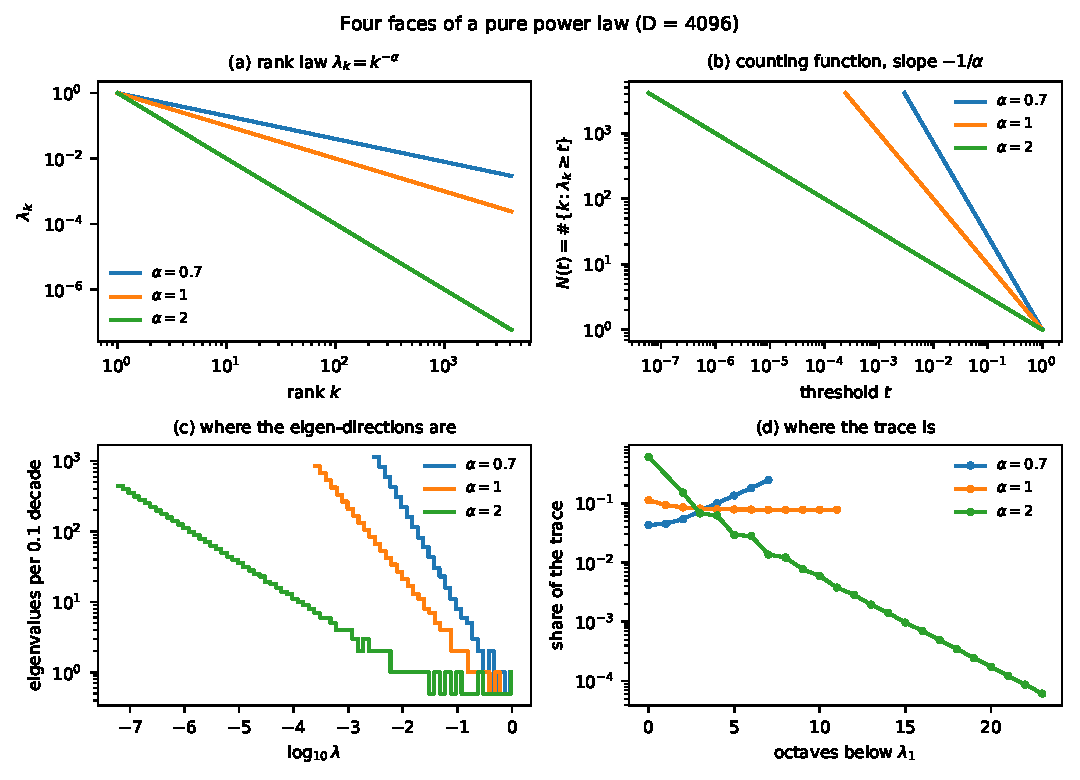
\includegraphics[width=\linewidth]{figures/faces.pdf}
\caption{Four faces of a pure power law $\lambda_k=k^{-\alpha}$, $D=4{,}096$ (synthetic). (a) The rank law.
(b) Its counting function, with slope $-1/\alpha$ (Proposition~\ref{prop:faces}). (c) Eigenvalues per 0.1 decade:
most eigen-directions sit near the bottom (Remark~\ref{rem:reading}). (d) Share of the trace per full octave below
$\lambda_1$: top-heavy for $\alpha=2$, flat for $\alpha=1$, bottom-heavy for $\alpha=0.7$
(Corollary~\ref{cor:alphaone}).}
\label{fig:faces}
\end{figure}

%======================================================================
\section{What the exponent decides}\label{sec:controls}
%======================================================================

\begin{lemma}[Power sums]\label{lem:sums}
Let $S_s(K)=\sum_{k=1}^K k^{-s}$.
\begin{enumerate}[(a)]
\item For $s>1$: $S_s(K)\le\zeta(s)$ and $\sum_{k>m}k^{-s}\le m^{1-s}/(s-1)$. The first $m$ ranks carry all but a
  fraction at most $m^{1-s}/((s-1)\zeta(s))$.
\item For $s=1$: $S_1(K)=H_K=\ln K+\gamma+O(1/K)$, and each dyadic block of ranks $\{2^j,\dots,2^{j+1}-1\}$
  contributes $\ln2+O(2^{-j})$.
\item For $0\le s<1$: $S_s(K)=K^{1-s}/(1-s)+O(1)$, and the ranks above $K/2$ carry a fraction $1-2^{s-1}+o(1)$.
  For $s<0$: $S_s(K)=K^{1-s}/(1-s)\,(1+o(1))$.
\end{enumerate}
\end{lemma}
\begin{proof}
For decreasing $f(x)=x^{-s}$ ($s\ge0$), $\int_m^{M+1}f\le\sum_{k=m}^Mf(k)\le f(m)+\int_m^Mf$. Each claim follows by
evaluating the integrals; for $s<0$ the terms increase and the inequalities reverse.
\end{proof}

\begin{corollary}[Which part of a pure law decides a trace functional]\label{cor:decides}
For $\lambda_k=c\,k^{-\alpha}$, $k=1,\dots,D$, we have $\tr A^q=c^qS_{\alpha q}(D)$, so
\begin{center}
\begin{tabular}{lccc}
\toprule
Functional & decided by the top when & marginal at & decided by the tail when\\
\midrule
$\tr A^2=\norm{A}_\F^2$ & $\alpha>1/2$ & $\alpha=1/2$ & $\alpha<1/2$\\
$\tr A$ & $\alpha>1$ & $\alpha=1$ & $\alpha<1$\\
$\tr A^{1/2}$ & $\alpha>2$ & $\alpha=2$ & $\alpha<2$\\
$\tr A^{-1}$ & never & --- & always ($\propto D^{1+\alpha}$)\\
\bottomrule
\end{tabular}
\end{center}
A fit on the head decides only the top-dominated entries. Tail-dominated quantities depend on the part of $\mu_A$ the
fit does not see: the trace for $\alpha<1$, and every negative power, which is what preconditioning uses.
\end{corollary}

\begin{corollary}[At $\alpha=1$ every octave carries the same trace]\label{cor:alphaone}
For a pure law with $\alpha=1$, every full octave of eigenvalues $[t,2t)$ carries trace $c\ln2+O(t)$. The top-$k$
share of the trace is $H_k/H_D\approx\ln k/\ln D$. For the top 16 it is \NumShareFourK{} at $D=4{,}096$,
\NumShareSixteenK{} at $D=16{,}384$ and \NumShareSixForty{} at $D=640$.
\end{corollary}
\begin{proof}
The eigenvalues in $[t,2t)$ have ranks $c/(2t)<k\le c/t$, and $\sum c/k$ over these ranks is $c\ln2+O(t)$ by
Lemma~\ref{lem:sums}(b). The share is $\sum_{k\le16}(c/k)/\sum_{k\le D}(c/k)$.
\end{proof}

\begin{observation}[The late trace is consistent with an $\alpha\approx1$ law; \evL]\label{obs:trace}
In \study{spectral_rotation_20261020} (raw per-tensor GGN on one fixed batch), the late fits (steps 250--500) give
$\alpha\approx0.9$--$1.1$ on ranks 1--200, with a slightly flatter head ($\alpha_{\text{top}}=0.65$--$0.86$) and
$\alpha_{\text{bulk}}=0.96$--$1.17$. The median top-16 share of the exact block trace over the 39 tensors is
0.35--0.45 at step 400 and 0.33--0.42 at step 500. A pure $\alpha=1$ law over all ranks gives \NumShareFourK{} for
the 24 blocks with $D=4{,}096$ and \NumShareSixteenK{} for the 12 with $D=16{,}384$. The trace is the only measured
quantity that sees the whole spectrum, and it is consistent with the law extending well below rank 200. It is one
number per tensor, so this is a consistency check, not a test.
\end{observation}

\begin{observation}[Spectra leave the law at the bottom; \evL]\label{obs:bottom}
In \study{noise_scale_20261021} the smallest Ritz value of a damped whitened block $K+\delta I$ was $0.9987\,\delta$,
so at least one block has eigenvalues at numerical zero. Measured spectra leave any power law at the bottom (finite
data, symmetries). The tail-dominated rows of Corollary~\ref{cor:decides} are then set by the damping, not by the law.
\end{observation}

\begin{proposition}[Effective dimension under damping]\label{prop:deff}
For $\delta>0$ let
\[d_\delta(A)=\tr A(A+\delta I)^{-1}=\sum_k\frac{\lambda_k}{\lambda_k+\delta}.\]
\begin{enumerate}[(a)]
\item For every $A\in\Sym^D_+$: $\tfrac12N_A(\delta)\le d_\delta(A)\le N_A(\delta)+\delta^{-1}\sum_{\lambda_k<\delta}\lambda_k$.
\item For a pure law with $\alpha>1$ and $D=\infty$:
  $\abs[\big]{d_\delta-(c/\delta)^{1/\alpha}\,\frac{\pi/\alpha}{\sin(\pi/\alpha)}}\le1$.
\item For a pure law with $\alpha=1$: $\abs[\big]{d_\delta-(c/\delta)\ln(1+D\delta/c)}\le1$.
\end{enumerate}
\end{proposition}
\begin{proof}
(a) Terms with $\lambda_k\ge\delta$ lie in $[1/2,1]$; terms with $\lambda_k<\delta$ are at most $\lambda_k/\delta$.
(b) $f(x)=1/(1+(\delta/c)x^\alpha)$ is decreasing with $f(0)=1$, so $\abs{\sum_{k\ge1}f(k)-\int_0^\infty f}\le1$, and
$\int_0^\infty dx/(1+ax^\alpha)=a^{-1/\alpha}\int_0^\infty du/(1+u^\alpha)=a^{-1/\alpha}(\pi/\alpha)/\sin(\pi/\alpha)$.
(c) The same comparison with $\int_0^Ddx/(1+\delta x/c)$.
\end{proof}
Numerical check: for $\alpha=2$ and $\delta=10^{-6}c$ the sum (to rank $10^7$) is \NumDdeltaExact{} against
\NumDdeltaAsym; for $\alpha=1$, $D=4{,}096$ and $\delta=10^{-3}c$ it is \NumDdeltaLogExact{} against
\NumDdeltaLogAsym. Damping $\delta$ effectively truncates the law at rank $N_A(\delta)=(c/\delta)^{1/\alpha}$. At
$\alpha=1$ the directions below $\delta$ still add a logarithmic factor, so the same damping keeps very different
numbers of directions active for different exponents.

%======================================================================
\section{The spectrum as a probability distribution}\label{sec:distribution}
%======================================================================

\subsection{Spectrum known, frame unknown}

\begin{definition}[The Haar model]\label{def:haar}
Fix $\Lambda$, draw $Q$ from the Haar (uniform) distribution on $\Orth(D)$, and set $A=Q\Lambda Q^\top$. The law of
$A$ is the unique probability distribution on $\mathcal{O}_\Lambda$ that is invariant under all rotations
$A\mapsto RAR^\top$. It models a matrix whose spectrum is known and whose frame is not.
\end{definition}

\begin{proposition}[The eigenvalue an unmeasured direction meets]\label{prop:haar}
In the Haar model, let $v$ be a fixed unit vector and $w_k=(q_k^\top v)^2$, with $q_k$ the columns of $Q$.
\begin{enumerate}[(a)]
\item $(w_1,\dots,w_D)\sim\Dir(\tfrac12,\dots,\tfrac12)$; in particular $\E w_k=1/D$.
\item Let $I$ be a random index with $\Pr(I=k\mid Q)=w_k$. Then $\Pr(I=k)=1/D$, so $\lambda_I\sim\mu_A$.
\item For every $f$, $v^\top f(A)v=\sum_kf(\lambda_k)w_k=\E[f(\lambda_I)\mid Q]$, and
\[
\E\bigl[v^\top f(A)v\bigr]=\int f\,d\mu_A,\qquad \Var\bigl[v^\top f(A)v\bigr]=\frac{2\Var_{\mu_A}(f)}{D+2}.
\]
\end{enumerate}
\end{proposition}
\begin{proof}
$Q^\top v$ is uniform on the unit sphere because $Q$ is Haar distributed. A uniform unit vector is $g/\norm{g}$ with
$g\sim\mathcal{N}(0,I_D)$. The $g_k^2$ are independent Gamma$(\frac12,2)$ variables, and independent Gamma variables
with a common scale, normalised by their sum, are Dirichlet distributed: this gives (a), and (b) follows from
$\E w_k=1/D$. For (c), the Dirichlet moments are $\Var w_k=2(D-1)/(D^2(D+2))$ and $\Cov(w_k,w_l)=-2/(D^2(D+2))$, so
$\Var\sum_kf_kw_k=\frac{2}{D^2(D+2)}\bigl(D\sum_kf_k^2-(\sum_kf_k)^2\bigr)=2\Var_{\mu_A}(f)/(D+2)$.
\end{proof}

\begin{example}\label{ex:haar}
For a pure $\alpha=1$ law with $D=4{,}096$, the Rayleigh quotient $v^\top Av$ of a uniformly random direction has mean
$\tr A/D$ and relative standard deviation \NumHaarRelSd. A Monte Carlo check (\NumHaarMCDraws{} draws, $D=256$)
reproduces the variance formula with ratio \NumHaarMCVarRatio{} and the mean with ratio \NumHaarMCMeanRatio.
\end{example}

\begin{remark}[The probabilistic-numerics reading]\label{rem:pn}
Proposition~\ref{prop:haar} is the precise sense in which ``the spectrum is a distribution''. When nothing is known
about the frame, $\mu_A$ is the prior predictive distribution of the curvature that any direction will meet. A
matrix--vector product $Av$ is an observation that changes this: it reveals part of the spectral measure seen from
$v$ (Section~\ref{sec:seen}). In the language of probabilistic numerics (Hennig 2015; Wenger \& Hennig 2020), the
spectrum plays the role of the prior, and computation, the products, is inference about the frame relative to the
vectors we care about. Part~III develops this.
\end{remark}

\subsection{The spectral measure seen from a vector}\label{sec:seen}

\begin{definition}
For $v\in\R^D$, the spectral measure of $A$ seen from $v$ is $\mu_{A,v}=\sum_k(u_k^\top v)^2\,\delta_{\lambda_k}$,
of total mass $\norm{v}^2$; its normalisation is $\nu_{A,v}=\mu_{A,v}/\norm{v}^2$.
\end{definition}

\begin{proposition}\label{prop:seen}
\begin{enumerate}[(a)]
\item $\int f\,d\mu_{A,v}=v^\top f(A)v$ for every $f$.
\item $\mu_{QAQ^\top,\,Qv}=\mu_{A,v}$ for all $Q\in\Orth(D)$.
\item In the Haar model, $\E\,\mu_{A,v}=\norm{v}^2\mu_A$ as measures.
\item (Golub \& Meurant 2010) Lanczos run for $m$ steps on $A$ from $v$ returns nodes $\theta_1,\dots,\theta_m$ and
  weights $\tau_1,\dots,\tau_m$ (the squared first components of the eigenvectors of its tridiagonal matrix) with
  $\sum_j\tau_j\theta_j^i=\int\lambda^i\,d\nu_{A,v}(\lambda)$ for $0\le i\le2m-1$: it computes the $m$-point Gauss
  quadrature rule of $\nu_{A,v}$.
\item For $A\succ0$, conjugate gradients on $Ax=b$ from $x_0=0$ satisfies
  \[\norm{x-x_m}_A^2=\min\Bigl\{\int p(\lambda)^2\lambda^{-1}\,d\mu_{A,b}(\lambda):\deg p\le m,\ p(0)=1\Bigr\}.\]
\end{enumerate}
\end{proposition}
\begin{proof}
(a) $A=\sum_k\lambda_ku_ku_k^\top$. (b) $QAQ^\top$ has eigenvectors $Qu_k$, and $(Qu_k)^\top Qv=u_k^\top v$.
(c) Proposition~\ref{prop:haar}(a). (d) Golub \& Meurant (2010). (e) CG's iterate $x_m=q(A)b$ minimises the $A$-norm
error over polynomials $q$ of degree less than $m$. With $p(\lambda)=1-\lambda q(\lambda)$,
$x-x_m=p(A)A^{-1}b$ and $\norm{x-x_m}_A^2=b^\top p(A)^2A^{-1}b=\int p^2\lambda^{-1}\,d\mu_{A,b}$.
\end{proof}
So the frame enters Krylov methods only through the weights of the start vector. Two matrices with different frames
but the same measure seen from $b$ produce the same CG errors. (The \texttt{weights} in the lab's
\path{noise_scale_20261021/scripts/lanczos.py} are exactly the $\tau_j$ of (d).)

\begin{proposition}[One step on a quadratic]\label{prop:step}
Let $A\succ0$, $g\in\R^D$ and $q(x)=\frac12x^\top Ax-g^\top x$. For $f>0$ on the spectrum, the best decrease along
$x=\alpha f(A)g$ is
\[
\max_\alpha\bigl[q(0)-q(\alpha f(A)g)\bigr]=\frac{\bigl(\int f\,d\mu_{A,g}\bigr)^2}{2\int\lambda f(\lambda)^2\,d\mu_{A,g}(\lambda)}.
\]
\end{proposition}
\begin{proof}
$q(\alpha f(A)g)=\frac12\alpha^2g^\top f(A)Af(A)g-\alpha g^\top f(A)g$. Maximise over $\alpha$ and use
Proposition~\ref{prop:seen}(a).
\end{proof}

\begin{corollary}[The value of curvature is a spread]\label{cor:kantorovich}
For Newton ($f=1/\lambda$) against a tuned gradient step ($f=1$), the ratio of best decreases is
$\E_\nu[\lambda]\,\E_\nu[\lambda^{-1}]$ with $\nu=\nu_{A,g}$. It lies in $[1,(\kappa+1)^2/(4\kappa)]$, with $\kappa$
the condition number on the support of $\nu$ (Kantorovich). For a vector with uniform spectral weights ($\nu=\mu_A$)
and a pure $\alpha=1$ law it equals $H_D(D+1)/(2D)\approx\frac12\ln D$: \NumKantFourK{} at $D=4{,}096$ and
\NumKantSixteenK{} at $D=16{,}384$.
\end{corollary}
\begin{proof}
Proposition~\ref{prop:step} gives
\[
\text{Newton: }\tfrac12\int\lambda^{-1}\,d\mu_{A,g},\qquad
\text{gradient: }\frac{\bigl(\int d\mu_{A,g}\bigr)^2}{2\int\lambda\,d\mu_{A,g}};
\]
divide. For the pure law, $\E_\mu[\lambda]=cH_D/D$ and $\E_\mu[\lambda^{-1}]=(D+1)/(2c)$.
\end{proof}

\begin{remark}[Two measures decide a step]\label{rem:twomeasures}
With batch noise of covariance $\Sigma$, the denominator of Proposition~\ref{prop:step} gains the term
$(1/B-1/N)\int\lambda f^2\,d\mu_{A,\Sigma}$, where $\mu_{A,\Sigma}=\sum_k(u_k^\top\Sigma u_k)\,\delta_{\lambda_k}$
(\texttt{batch\_noise.md}, T1). For one step, all that matters about $A$ is the pair $(\mu_{A,\bar g},\mu_{A,\Sigma})$:
how the signal and the noise are spread over the spectrum. The frame enters only through these weights. Two questions
follow for training. Does the gradient's measure $\nu_{A,\bar g}$ stay stationary while the frame rotates, that is,
does the gradient co-rotate with the frame? And how do it and $\mu_{A,\Sigma}$ change during training? The forms
$z^\top A^qz$, $q\in[-1,1]$, measured in \study{noise_scale_20261021} are moments of exactly these measures.
\end{remark}

%======================================================================
\section{What a power law implies about the frame}\label{sec:resolution}
%======================================================================

\begin{proposition}[Eigenvalues are stable]\label{prop:weyl}
For $A,B\in\Sym^D$ with sorted eigenvalues:
\begin{enumerate}[(a)]
\item $\abs{\lambda_k(A)-\lambda_k(B)}\le\norm{A-B}_\op$ for every $k$ (Weyl);
\item $\sum_k(\lambda_k(A)-\lambda_k(B))^2\le\norm{A-B}_\F^2$ (Hoffman--Wielandt);
\item hence $W_2(\mu_A,\mu_B)\le\norm{A-B}_\F/\sqrt D$.
\end{enumerate}
\end{proposition}
\begin{proof}
(a) and (b): Bhatia (1997). (c) On the real line the monotone coupling is optimal for the Wasserstein-2 distance, so
$W_2(\mu_A,\mu_B)^2=D^{-1}\sum_k(\lambda_k(A)-\lambda_k(B))^2$.
\end{proof}

\begin{proposition}[Eigenvectors are only as stable as their gaps]\label{prop:dk}
(Davis--Kahan, in the form of Yu, Wang \& Samworth 2015.) Let $A,B\in\Sym^D$, $E=B-A$, and
$g_k=\min(\lambda_{k-1}(A)-\lambda_k(A),\,\lambda_k(A)-\lambda_{k+1}(A))>0$ with $\lambda_0=+\infty$,
$\lambda_{D+1}=-\infty$. Then $\sin\angle(u_k(A),u_k(B))\le2\norm{E}_\op/g_k$. For the top-$k$ subspaces,
$\norm{\sin\Theta}_\F\le2\min(\sqrt k\norm{E}_\op,\norm{E}_\F)/(\lambda_k(A)-\lambda_{k+1}(A))$.
\end{proposition}

\begin{lemma}[Gaps of a power law]\label{lem:gaps}
If $\lambda_k=c\,k^{-\alpha}$, then $\frac{\alpha}{k}(1+\frac1k)^{-\alpha-1}\le(\lambda_k-\lambda_{k+1})/\lambda_k\le\frac{\alpha}{k}$,
and for $2\le k<D$ the gap $g_k$ of Proposition~\ref{prop:dk} equals $\lambda_k-\lambda_{k+1}$.
\end{lemma}
\begin{proof}
$h(x)=1-(1+x)^{-\alpha}$ is concave with $h(0)=0$ and $h'(x)=\alpha(1+x)^{-\alpha-1}$, so $xh'(x)\le h(x)\le xh'(0)$;
take $x=1/k$. The map $k\mapsto c\,k^{-\alpha}$ is convex and decreasing, so consecutive gaps decrease and the gap
below is the smaller one.
\end{proof}

\begin{proposition}[Two resolution limits]\label{prop:resolution}
Let $A$ follow a pure law $(c,\alpha)$ and $\norm{B-A}_\op\le\eta$. For $s\in(0,1]$:
\begin{enumerate}[(a)]
\item $\abs{\lambda_k(B)-\lambda_k(A)}\le s\lambda_k(A)$ for every $k\le K_{\text{val}}:=(sc/\eta)^{1/\alpha}$;
\item $\sin\angle(u_k(A),u_k(B))\le s$ for every $k<D$ with $k\le K_{\text{vec}}:=\bigl(s\alpha c/(2^{\alpha+2}\eta)\bigr)^{1/(\alpha+1)}$;
\item $K_{\text{vec}}/K_{\text{val}}\to0$ as $\eta\to0$: for small perturbations far more eigenvalues are resolved
  than eigenvectors.
\end{enumerate}
\end{proposition}
\begin{proof}
(a) Weyl: $\abs{\Delta\lambda_k}\le\eta\le sc\,k^{-\alpha}$ if and only if $k\le(sc/\eta)^{1/\alpha}$.
(b) By Lemma~\ref{lem:gaps} and $1+1/k\le2$, $g_k\ge\alpha c\,k^{-\alpha-1}2^{-\alpha-1}$ (for $k=1$ the gap is
$\lambda_1-\lambda_2$, covered by the same bound). Proposition~\ref{prop:dk} gives
$\sin\le2\eta/g_k\le2^{\alpha+2}\eta k^{\alpha+1}/(\alpha c)\le s$ for $k\le K_{\text{vec}}$.
(c) $K_{\text{vec}}/K_{\text{val}}\propto\eta^{1/\alpha-1/(\alpha+1)}=\eta^{1/(\alpha(\alpha+1))}\to0$.
\end{proof}

These are worst-case guarantees. Typical perturbations behave alike, with explicit constants.

\begin{approximation}[Typical perturbations]\label{approx:typical}
Let $E$ have independent centred Gaussian entries, with variance $\varepsilon^2$ off the diagonal and $2\varepsilon^2$
on it, so that $\norm{E}_\op\approx2\varepsilon\sqrt D$. While the result is small, first-order perturbation theory
gives
\[
\sin^2\angle(u_k(A),u_k(B))\approx\varepsilon^2\sum_{j\ne k}(\lambda_k-\lambda_j)^{-2}.
\]
For a pure law the sum has two parts. The neighbouring ranks contribute
$\sum_{m\ne0}(mg_k)^{-2}\approx2\zeta(2)k^{2\alpha+2}/(\alpha^2c^2)$, and the many much smaller eigenvalues about
$Dk^{2\alpha}/c^2$. The neighbours dominate for $k\gtrsim\alpha\sqrt{D/(2\zeta(2))}$. The typical eigenvector
resolution limit, where the sine reaches $s$, is then
\[
k_{\text{vec}}\approx\Bigl(\frac{s\alpha c}{\sqrt{2\zeta(2)}\,\varepsilon}\Bigr)^{1/(\alpha+1)}.
\]
An isolated eigenvalue moves by about $\sqrt2\varepsilon$ (its diagonal entry), and no eigenvalue moves by more than
$\norm{E}_\op$.
\end{approximation}

Figure~\ref{fig:resolution} checks this for a pure $\alpha=1$ law with $D=\NumSimDim$ and $\varepsilon=10^{-5}$
($\norm{E}_\op\approx\NumSimEtaScaled\times10^{-4}$; medians of three draws).
\begin{itemize}
\item \emph{Eigenvalues:} relative errors stay below $\NumRelValTopScaled\times10^{-3}$ in the top 100 ranks and reach
  0.5 only at rank \NumKvalSim{} (Weyl's worst case: rank \NumKvalWeyl).
\item \emph{Eigenvectors:} the first-order formula matches the simulated angles, and the sine reaches 0.5 at rank
  \NumKvecSim{} (predicted \NumKvecPred).
\end{itemize}
Eigenvalues are resolved about ten times deeper than eigenvectors here.

\begin{proposition}[Lipschitz spectral functions are as stable as the matrix]\label{prop:lipschitz}
If $f$ is $L$-Lipschitz on an interval containing the spectra of $A,B\in\Sym^D$, then
$\norm{f(A)-f(B)}_\F\le L\norm{A-B}_\F$.
\end{proposition}
\begin{proof}
Write $A=U_A\Lambda_AU_A^\top$, $B=U_B\Lambda_BU_B^\top$ and $W=U_A^\top U_B$. Then $U_A^\top(A-B)U_B=\Lambda_AW-W\Lambda_B$
has entries $(a_i-b_j)W_{ij}$, and $U_A^\top(f(A)-f(B))U_B$ has entries $(f(a_i)-f(b_j))W_{ij}$. Since
$\abs{f(a_i)-f(b_j)}\le L\abs{a_i-b_j}$ entrywise and the Frobenius norm is invariant under orthogonal factors, the
claim follows.
\end{proof}

\begin{corollary}[Damping sets the stability of a fractional step]\label{cor:fractional}
$f(\lambda)=(\lambda+\delta)^{-\nu}$ is $\nu\delta^{-\nu-1}$-Lipschitz on $[0,\infty)$, so
$\norm{(A+\delta I)^{-\nu}-(B+\delta I)^{-\nu}}_\F\le\nu\delta^{-\nu-1}\norm{A-B}_\F$, whatever the eigenvectors
did. The top-$k$ projector $\Pi_k$ has no bound of this kind. By Proposition~\ref{prop:dk},
$\norm{\Pi_k(A)-\Pi_k(B)}_\F=\sqrt2\norm{\sin\Theta}_\F\le2\sqrt2\min(\sqrt k\norm{E}_\op,\norm{E}_\F)/(\lambda_k-\lambda_{k+1})$,
and for a power law the gap at the cut is about $\alpha\lambda_k/k$ (Lemma~\ref{lem:gaps}).
\end{corollary}

\begin{remark}[A cut or a smooth function?]\label{rem:cut}
The two bounds have different strengths, and Figure~\ref{fig:resolution}c shows both effects. A hard cut where the
gap is large is far more stable than a smooth ``soft cut'' $A(A+\lambda_kI)^{-1}$ at the same place: at $k=16$ the
relative errors are \NumHardSixteen{} (hard) and \NumSoftSixteen{} (soft). The smooth function acts on every
direction and pays for the perturbation everywhere; its error is controlled by $\norm{E}_\F$, which grows like
$\varepsilon D$. Deep in the spectrum, where gaps are tiny, the order reverses: at $k\approx1{,}000$ the errors are
\NumHardThousand{} (hard) and \NumSoftThousand{} (soft). The curves cross at $k\approx\NumCrossCut$, about twice the
eigenvector resolution limit. (Soft-cut values are on a grid of cut positions; the ones quoted are at
\NumSoftCuts.)

The design rule this suggests is not ``never store a frame'' but: cut only where the frame is resolved, and use
smooth functions of the current matrix beyond that. PARSEC-L's brake
$I-\sum_{k\le r}\frac{\kappa_k}{1+\kappa_k}w_kw_k^\top$ with $\kappa_k=c_{\mathrm b}\eta\lambda_k$ is exactly the
soft function $\lambda/(\lambda+1/(c_{\mathrm b}\eta))$ applied inside a hard top-$r$ cut. Its fully smooth version is
$(I+c_{\mathrm b}\eta K)^{-1}$, which needs no eigenvectors.
\end{remark}

\begin{figure}[t]
\centering
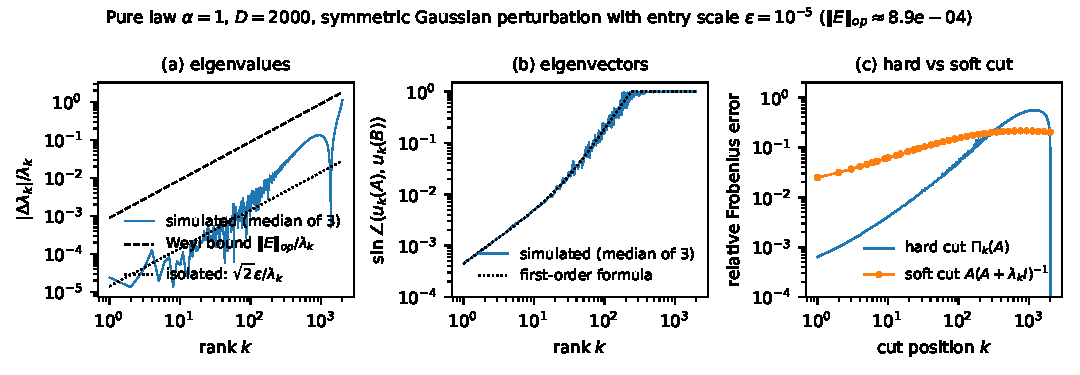
\includegraphics[width=\linewidth]{figures/resolution.pdf}
\caption{Resolution limits (synthetic). A pure $\alpha=1$ law, $D=\NumSimDim$, perturbed by a symmetric Gaussian
matrix with entry scale $\varepsilon=10^{-5}$; medians of three draws. (a) Relative eigenvalue errors, with Weyl's
bound and the isolated-eigenvalue estimate $\sqrt2\varepsilon/\lambda_k$. (b) Eigenvector angles, with the
first-order formula of Approximation~\ref{approx:typical}. (c) Relative Frobenius error of the top-$k$ projector (hard
cut) and of the soft cut $A(A+\lambda_kI)^{-1}$ at the same place (Remark~\ref{rem:cut}).}
\label{fig:resolution}
\end{figure}

\begin{proposition}[Stale frame, fresh diagonal]\label{prop:pinching}
Let $U\in\Orth(D)$ be any frame, for example the eigenframe of an earlier matrix, and let $A\in\Sym^D$. Define the
pinching $\mathcal{P}_U(A)=U\diag(u_1^\top Au_1,\dots,u_D^\top Au_D)\,U^\top$.
\begin{enumerate}[(a)]
\item $\mathcal{P}_U(A)$ is the closest matrix to $A$ in Frobenius norm among matrices with frame $U$, and
  $\norm{A-\mathcal{P}_U(A)}_\F^2=\sum_{i\ne j}(u_i^\top Au_j)^2$.
\item $\tr\mathcal{P}_U(A)=\tr A$, and the eigenvalues of $\mathcal{P}_U(A)$, the Rayleigh quotients $u_i^\top Au_i$,
  are majorised by those of $A$. For every $k$, the sum of the $k$ largest Rayleigh quotients is at most
  $\lambda_1(A)+\dots+\lambda_k(A)$. In particular $\max_iu_i^\top Au_i\le\lambda_1(A)$ and
  $\min_iu_i^\top Au_i\ge\lambda_D(A)$.
\end{enumerate}
\end{proposition}
\begin{proof}
(a) $U^\top(A-UMU^\top)U=U^\top AU-M$ for diagonal $M$: the off-diagonal part is fixed, and the diagonal part
vanishes for $M=\diag(U^\top AU)$. (b) Schur's theorem: the diagonal of a symmetric matrix is majorised by its
eigenvalues (Horn \& Johnson 2013, Section~4.3).
\end{proof}

\begin{remark}[The bridge to SOAP]\label{rem:soap}
This is the structure of EKFAC and SOAP: a frame refreshed rarely and a diagonal refreshed every step. Part (a) is
the Frobenius-optimality argument that George et al.\ (2018) give for EKFAC's diagonal, and Eschenhagen et al.\
(2025) analyse Shampoo and SOAP in the same Frobenius terms. Part (b) adds what a stale frame costs spectrally: the
effective spectrum is flattened, with the top lowered and the bottom raised, the more so the further the frame has
drifted. That is the direction of the shrinkage that rotationally invariant estimators from random-matrix statistics
apply when eigenvectors are unreliable (Bun, Bouchaud \& Potters 2017). Two cautions for Part~III: SOAP's diagonal
is an exponential average of squared rotated gradients, a second moment of the gradient rather than the GGN; and it
enters through a square root.
\end{remark}

\begin{observation}[Late rotation is not only near-tie mixing; \evL]\label{obs:rotation}
Late in training, the 10-step capture of a cached top-$k$ subspace rises with $k$: 0.78--0.84 at $k=1$ and
0.87--0.91 at $k=200$ (\study{spectral_rotation_20261020}). The study read this as mixing within nearly tied
groups, which is what Proposition~\ref{prop:resolution} and Approximation~\ref{approx:typical} predict for a power
law. But the late head is flatter ($\alpha_{\text{top}}=0.65$--$0.86$), so the relative gap below the top eigenvalue is
$1-2^{-\alpha_{\text{top}}}\approx0.36$--$0.45$, which is not small. Losing 16--22\% of the top direction's curvature
in 10 steps therefore means the 10-step change is not small compared with the top gap. Part~II has to allow
changes that are large at the top, not only mixing among near-ties. Rotation also exceeds batch noise: at fixed
weights another batch's top-16 subspace captures 0.93--0.999.
\end{observation}

%======================================================================
\section{What is known, and what is not (searches of 23 October 2026)}\label{sec:known}
%======================================================================

The motivating question was whether SOAP was built from a model of how spectrum and frame evolve. References marked
$^*$ were checked online on 23 October 2026, at least at the level of the abstract; the others are cited from memory.

\begin{itemize}
\item \textbf{EKFAC} (George et al.\ 2018$^*$). The eigenbasis is expensive and is recomputed rarely; the diagonal
  scaling in that basis is cheap and tracked every step. The justification is cost plus a Frobenius-norm argument
  (a provably better approximation of the Fisher than K-FAC). There is no model of how the eigenbasis moves.
\item \textbf{SOAP} (Vyas et al.\ 2024$^*$). Shampoo with power $1/2$ equals Adafactor in Shampoo's eigenbasis, and
  SOAP runs Adam there instead. The eigenbasis is described as slowly changing, and the second moments as cheap
  enough to update every step. The refresh interval (1--100) is studied empirically: SOAP degrades more slowly with
  it than Shampoo does. There is no model of eigenbasis drift against eigenvalue drift and no theory of the optimal
  interval. Momentum is kept in parameter space and projected into the current basis at every step; the second-moment
  estimate lives in the rotated space and, on our reading of their Algorithm~3, is not re-rotated when the basis
  changes (to be verified). Vyas et al.\ note that Anil et al.\ (2020, Appendix~B) described an essentially equivalent
  algorithm.
\item \textbf{Purifying Shampoo} (Eschenhagen et al.\ 2025$^*$). A Frobenius-norm view of Shampoo's heuristics. It
  decouples the updates of eigenvalues and eigenbasis, shows that correcting the eigenvalues replaces learning-rate
  grafting, and proposes an adaptive criterion for recomputing the eigenbasis, based on the termination rule of a
  warm-started QR iteration. This is the closest existing work to adaptive refreshing. Its criterion controls the
  current approximation error; it does not forecast the error from a model of the frame's motion.
\item \textbf{Power-law Hessian spectra.} Xie et al.\ (2022$^*$) report rank laws $\lambda_i\propto i^{-s}$ with
  $s\approx1$ in well-trained networks and give a maximum-entropy explanation; Tang et al.\ (2025$^*$) extend this to
  CNNs and LLMs. Meterez et al.\ (2026), the owner's reference for the ``stable law, rotating eigenvectors'' picture,
  was not found by our searches and is unverified here.
\item \textbf{Eigenvector dynamics in training.} Gur-Ari, Roberts \& Dyer (2018) find gradients concentrated in the
  top Hessian subspace. Marjankowska, Modugno \& Barucca (2026$^*$) track the displacement and localisation of leading
  Hessian eigenvectors under SGD and Adam; they do not connect it to spectral stability or to SOAP.
\item \textbf{Random-matrix statistics.} Rotationally invariant estimators keep the sample eigenvectors and replace
  the eigenvalues by a nonlinear shrinkage computed from the spectrum (Ledoit \& P\'ech\'e 2011; Bun et al.\
  2016$^*$; Bun, Bouchaud \& Potters 2017$^*$). Allez \& Bouchaud (2012) study eigenvector dynamics of exponentially
  weighted covariance matrices, the estimator family of SOAP's statistics. We found no connection to SOAP or
  Shampoo.
\item \textbf{Probabilistic numerics.} Gaussian inference on Hessians (Hennig \& Kiefel 2013; Hennig 2015), active
  inference of a preconditioner from noisy Hessian-vector products (de Roos \& Hennig 2019$^*$), calibrated
  probabilistic linear solvers (Wenger \& Hennig 2020), and the bias of mini-batch quadratics (Tatzel, Mucs\'anyi,
  Hackel \& Hennig 2025$^*$).
\end{itemize}

\paragraph{Conclusion.} As far as these searches show, no published work treats the spectral law as (nearly)
stationary and the frame as a latent process, and derives SOAP's refresh schedule, averaging windows or treatment of
momentum from such a model. Searches can miss work; this should be re-checked before any claim of novelty.

%======================================================================
\section{Where Part II starts}\label{sec:next}
%======================================================================

\paragraph{Plan for Part II (dynamics).}
\begin{enumerate}[(1)]
\item \emph{Identity:} split a change of $A$ into a spectral part and a rotation. With $W=U^\top\dot U$
  skew-symmetric, $U^\top\dot AU=\dot\Lambda+W\Lambda-\Lambda W$: the diagonal holds $\dot\lambda_k$ and the
  off-diagonal $(\lambda_j-\lambda_i)W_{ij}$. ``Stable spectrum'' means the change is nearly all off-diagonal.
\item \emph{Three stochastic pictures with different fingerprints.}
  \begin{itemize}
  \item Isotropic matrix noise (Dyson Brownian motion): eigenvector pairs diffuse at rates $\propto(\lambda_i-\lambda_j)^{-2}$.
  \item Frame diffusion (Brownian motion on $\Orth(D)$): rates independent of the gaps.
  \item Deterministic drift: ballistic, hence predictable.
  \end{itemize}
  Their fingerprints are capture against lag (linear or quadratic onset), rotation against gap, and replicas forked
  with different data orders.
\item \emph{Structure:} the change of a GGN under a weight step is not isotropic; what is its structure?
\item \emph{Data:} \study{spectral_rotation_20261020} saved spectra and captures. Replays (10--12 minutes per
  trajectory) give eigenvectors. \study{noise_scale_20261021}'s forms give the moments of the gradient's and the
  noise's spectral measures at 36 states without new compute.
\end{enumerate}

\paragraph{Questions for us.}
\begin{question}
Which matrix should the theory treat first: the GGN, which we measured, or SOAP's own statistic, Kronecker factors of
gradient second moments (Remark~\ref{rem:kron})?
\end{question}
\begin{question}
Is a scale-free law the right null hypothesis, given that the trace grows 1.3--1.6$\times$ during the learning-rate
decay while the shape does not (\study{spectral_rotation_20261020})?
\end{question}
\begin{question}
Which prior on the frame: uniform (Haar), or concentrated around SOAP's current basis (a matrix Bingham or
von~Mises--Fisher law)?
\end{question}
\begin{question}
Which first measurement: rotation against gap from replays, or the gradient's spectral measure, which the forms
saved by \study{noise_scale_20261021} give for free?
\end{question}

%======================================================================
\begin{thebibliography}{99}\setlength{\itemsep}{2pt}\small
\bibitem{allez} R.~Allez and J.-P.~Bouchaud. Eigenvector dynamics: general theory and some applications.
  \emph{Physical Review E} 86, 046202, 2012.
\bibitem{anil} R.~Anil, V.~Gupta, T.~Koren, K.~Regan and Y.~Singer. Scalable second order optimization for deep
  learning. arXiv:2002.09018, 2020.
\bibitem{bhatia} R.~Bhatia. \emph{Matrix Analysis}. Springer, 1997.
\bibitem{bunrie} J.~Bun, R.~Allez, J.-P.~Bouchaud and M.~Potters. Rotational invariant estimator for general noisy
  matrices. \emph{IEEE Transactions on Information Theory}, 2016. arXiv:1502.06736.$^*$
\bibitem{bun} J.~Bun, J.-P.~Bouchaud and M.~Potters. Cleaning large correlation matrices: tools from random matrix
  theory. \emph{Physics Reports} 666, 2017. arXiv:1610.08104.$^*$
\bibitem{deroos} F.~de Roos and P.~Hennig. Active probabilistic inference on matrices for pre-conditioning in
  stochastic optimization. \emph{AISTATS}, PMLR 89:1448--1457, 2019. arXiv:1902.07557.$^*$
\bibitem{eschenhagen} R.~Eschenhagen, A.~Defazio, T.-H.~Lee, R.~E.~Turner and H.-J.~M.~Shi. Purifying Shampoo:
  investigating Shampoo's heuristics by decomposing its preconditioner. \emph{NeurIPS}, 2025. arXiv:2506.03595.$^*$
\bibitem{george} T.~George, C.~Laurent, X.~Bouthillier, N.~Ballas and P.~Vincent. Fast approximate natural gradient
  descent in a Kronecker-factored eigenbasis. \emph{NeurIPS}, 2018. arXiv:1806.03884.$^*$
\bibitem{golub} G.~H.~Golub and G.~Meurant. \emph{Matrices, Moments and Quadrature with Applications}. Princeton
  University Press, 2010.
\bibitem{gurari} G.~Gur-Ari, D.~A.~Roberts and E.~Dyer. Gradient descent happens in a tiny subspace.
  arXiv:1812.04754, 2018.
\bibitem{hennig15} P.~Hennig. Probabilistic interpretation of linear solvers. \emph{SIAM Journal on Optimization}
  25(1), 2015.
\bibitem{hennigkiefel} P.~Hennig and M.~Kiefel. Quasi-Newton methods: a new direction. \emph{Journal of Machine
  Learning Research} 14, 2013.
\bibitem{horn} R.~A.~Horn and C.~R.~Johnson. \emph{Matrix Analysis}, 2nd edition. Cambridge University Press, 2013.
\bibitem{ledoit} O.~Ledoit and S.~P\'ech\'e. Eigenvectors of some large sample covariance matrix ensembles.
  \emph{Probability Theory and Related Fields} 151, 2011.
\bibitem{marjankowska} M.~Marjankowska, V.~Modugno and P.~Barucca. Characterizing optimizer-dependent training
  dynamics through Hessian eigenvector displacement and localization. HiLD workshop at ICML, 2026.
  arXiv:2606.30226.$^*$
\bibitem{tang} Tang et al. Investigating the overlooked Hessian structure: from CNNs to LLMs. \emph{ICML}, PMLR 267,
  2025.$^*$
\bibitem{tatzel} L.~Tatzel, B.~Mucs\'anyi, O.~Hackel and P.~Hennig. Debiasing mini-batch quadratics for applications
  in deep learning. \emph{ICLR}, 2025. arXiv:2410.14325.$^*$
\bibitem{vyas} N.~Vyas, D.~Morwani, R.~Zhao, I.~Shapira, D.~Brandfonbrener, L.~Janson and S.~Kakade. SOAP: improving
  and stabilizing Shampoo using Adam. arXiv:2409.11321, 2024 (ICLR 2025).$^*$
\bibitem{wenger} J.~Wenger and P.~Hennig. Probabilistic linear solvers for machine learning. \emph{NeurIPS}, 2020.
\bibitem{xie} Z.~Xie et al. On the power-law Hessian spectrums in deep learning. arXiv:2201.13011, 2022.$^*$
\bibitem{yu} Y.~Yu, T.~Wang and R.~J.~Samworth. A useful variant of the Davis--Kahan theorem for statisticians.
  \emph{Biometrika} 102(2), 2015.
\end{thebibliography}

\end{document}
